% \textbf{\underline{OZ 10 - De vergelijkingen van Maxwell + Herhalingsoefeningen - Oefening 2:}}
% \vspace{0.5cm}

% (\hyperref[OZ4:3]{Oefenzitting 4, oefening 3}) Een geleider die een stroom $ 2I $ draagt, splitst zich in twee (Figuur 10.1). Elke afgesplitste geleider draagt een stroom $ I $. Bereken de $ y $-component van het magnetische veld in het punt $ P $ als functie van $ \theta $ en $ a $. Ter verduidelijking: $ 2I $ stroomt langs de $ x $-as en splitst in het $ xy $-vlak. $ P $ ligt op de $ z $-as. (Hint: reken eerst $ \vec{B} $ uit in $ P $ van een stuk geleider met lengte $ L $.)

% \begin{figure}[H]
%     \centering
%     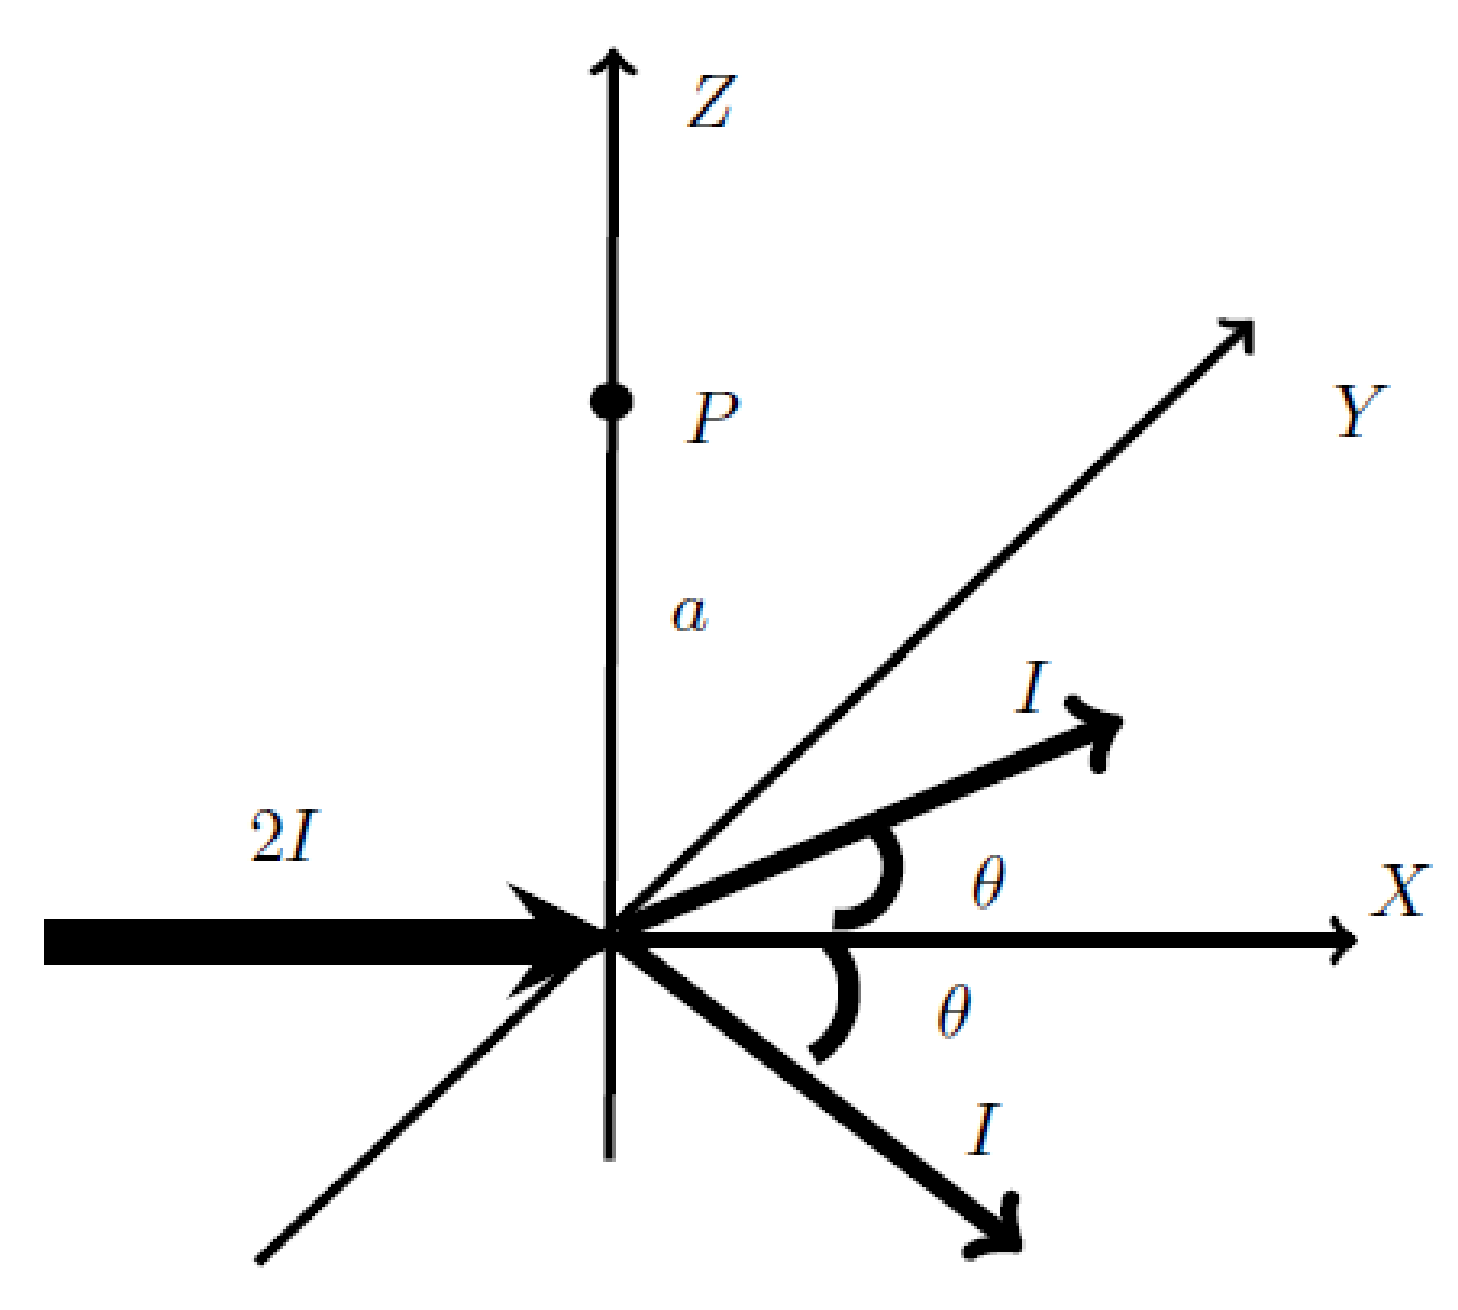
\includegraphics[width=5cm]{oz04/resources/oef-3-opgave.png}
    
%     \textbf{Figuur 10.1}
% \end{figure}

% \hyperref[OZ4:3]{Klik hier om de uitwerking te bekijken}

% \vspace{1cm}